\documentclass[12pt, letterpaper]{scrartcl}

\usepackage{fullpage} % Set margins and place page numbers at bottom center
\usepackage[shortlabels]{enumitem} % Use a. in the enumerate
\usepackage{amsmath} % aligned equations
\usepackage{graphicx} % include figure
\usepackage{float} % usage of H for figure float
\usepackage{amssymb} % \blacksqure and \triangleq
\usepackage{xcolor} % color in math mode

\usepackage[T1]{fontenc}
\usepackage[numbered,framed]{matlab-prettifier}
\lstset{
  style              = Matlab-editor,
  basicstyle         = \mlttfamily,
  escapechar         = ",
  mlshowsectionrules = true,
}

\begin{document}

% ### Header - start ###
    \begin{center}
    	\hrule
    	\vspace{0.4cm}
    	{\textbf { {\large Homework 5 + Population Bounds} \\ EE 668 --- Information Theory}}
    \end{center}
    { \textbf{Name:} Ali Zafari \hspace{\fill} \textbf{Student Number:} 800350381 \hspace{\fill} \textbf{Fall 2022} } \newline\hrule
% ### Header - end ###

\paragraph*{Population Bounds} \hfill\newline
Population bounds have been plotted as shown below, for binary codewords of length $n=245$. If there were no constraint (requiring a minimum distance between codes) on assigning codewords, $2^{245}$ codes can be imagined. But with the constraint on having minimum distance between them, this number quickly drops down below $2^{120}$ ($\approx 10^{36}$).  
\begin{figure}[H]
    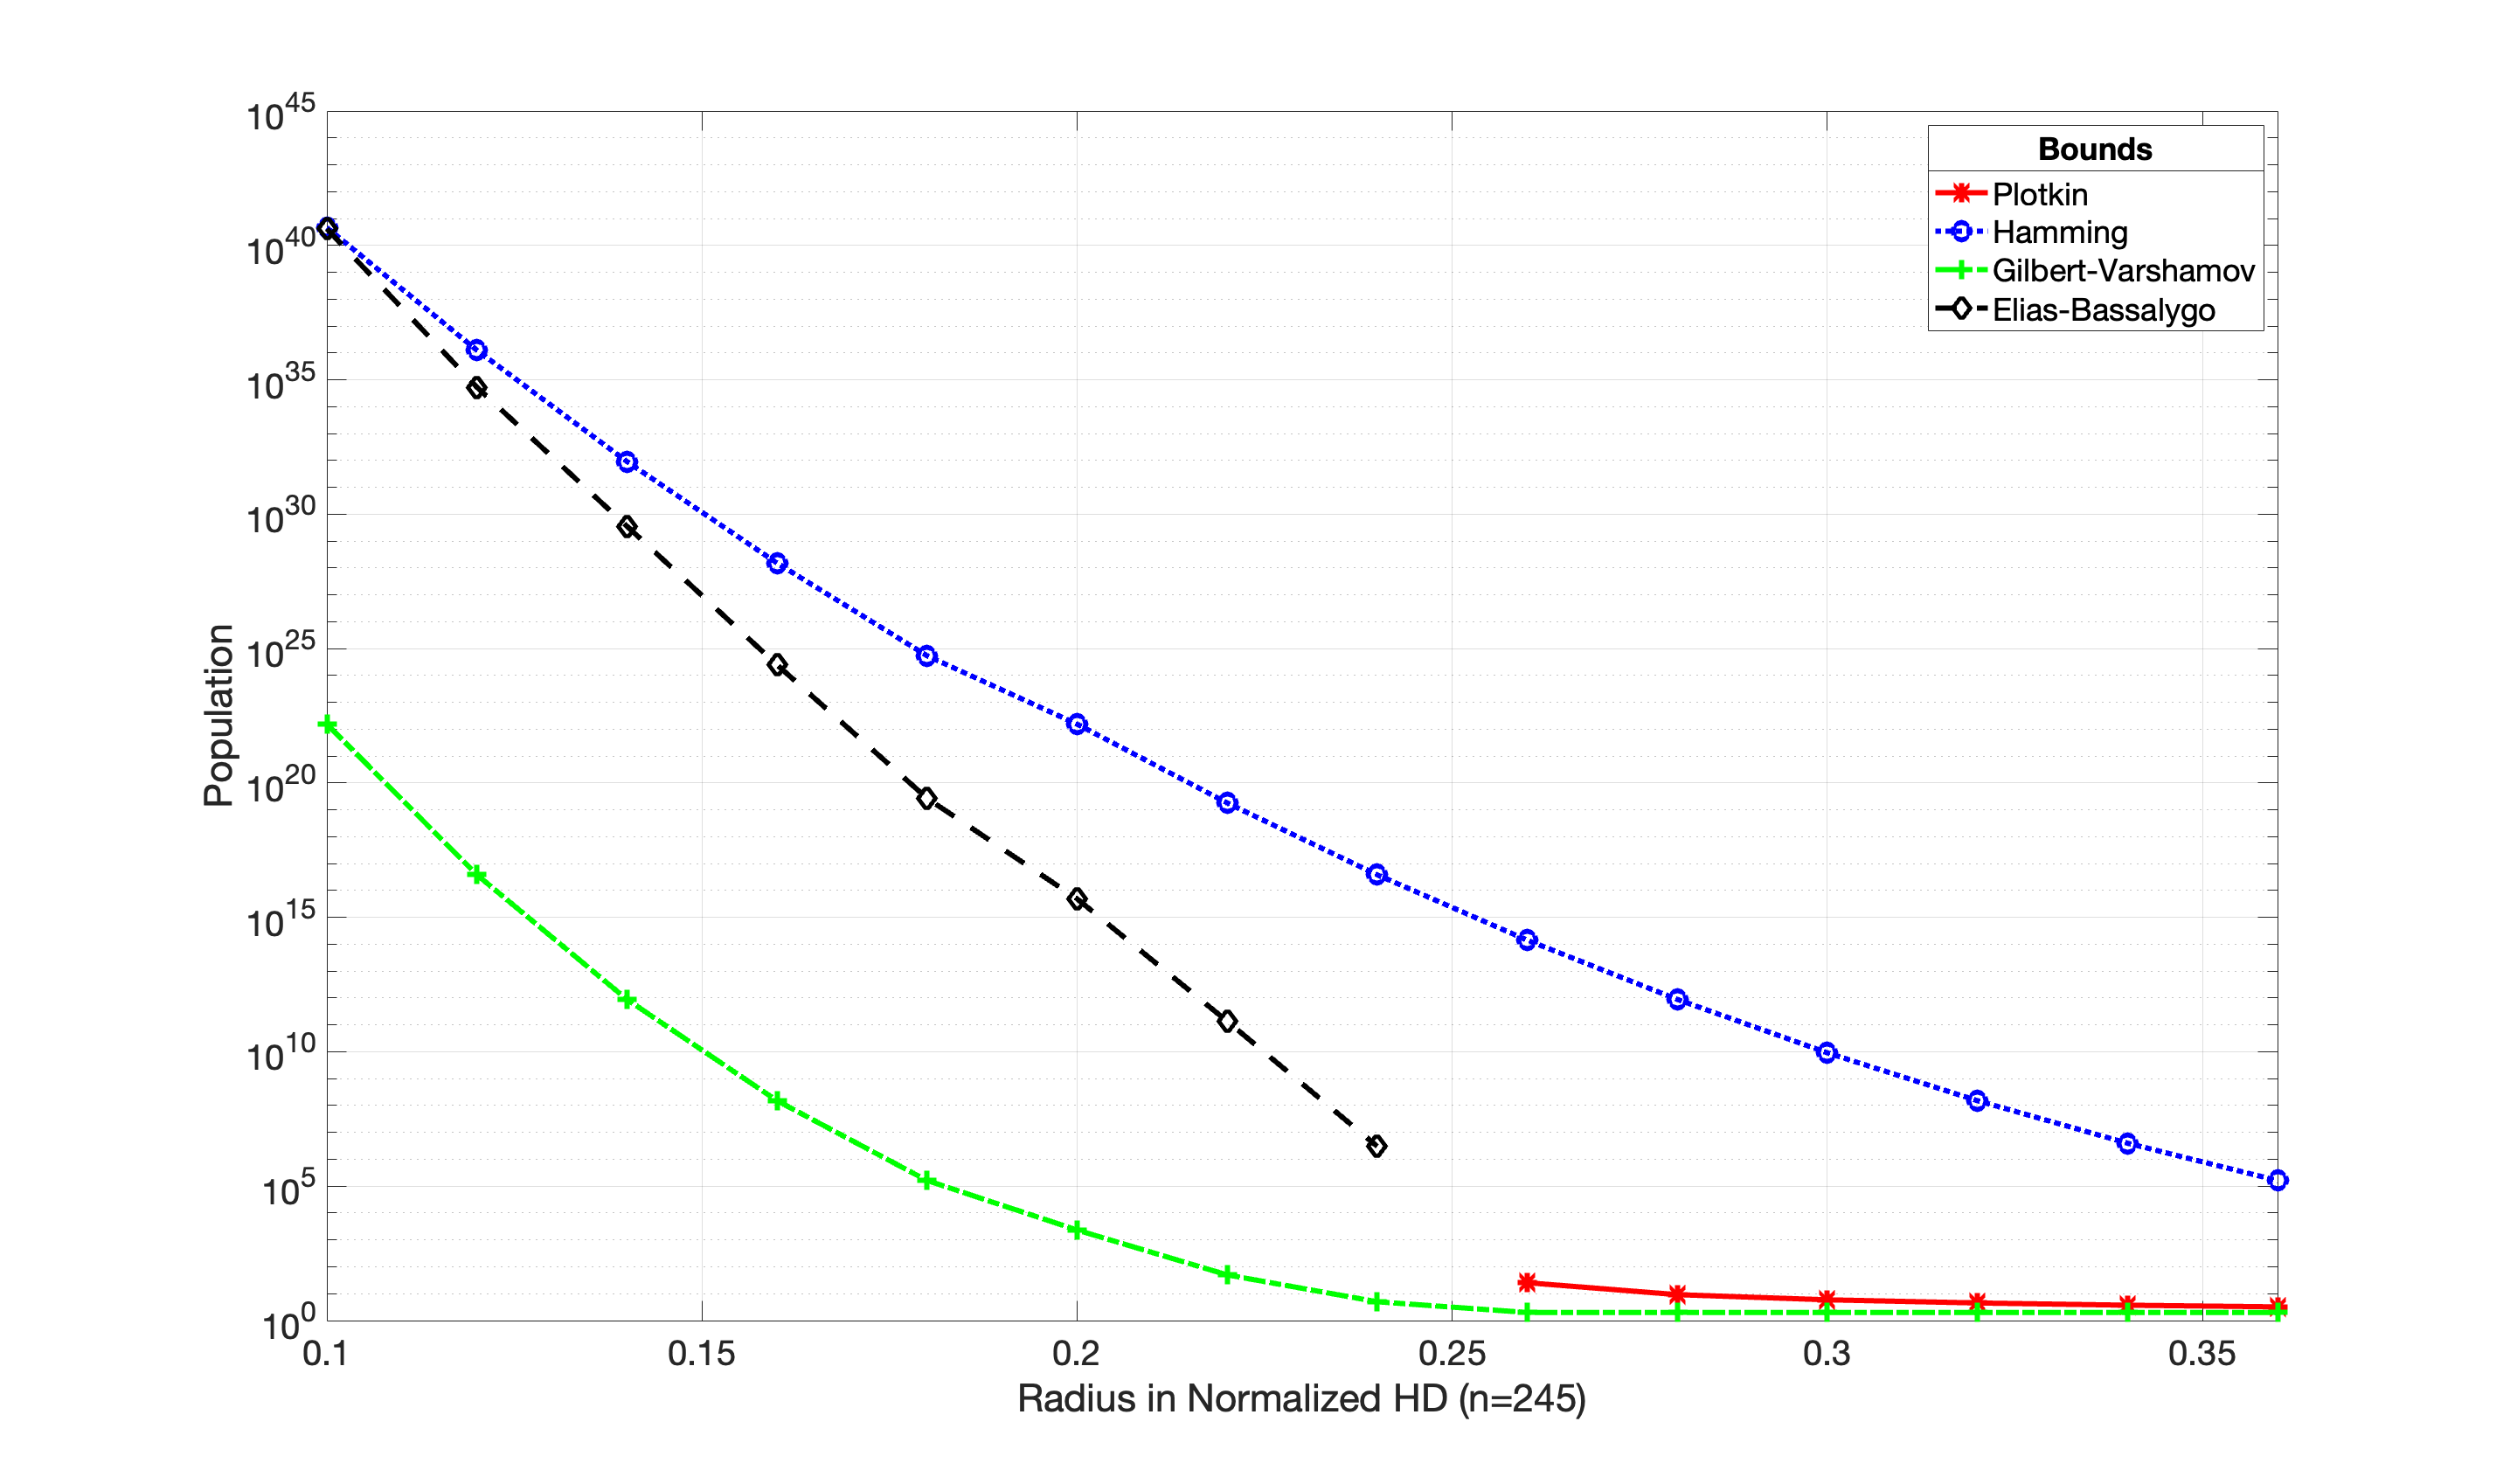
\includegraphics[width=\linewidth]{hw5_figures/245.png}
    \centering
    \caption{Population bounds vs. normalized Hamming distance ($n=245$)}
\end{figure}

For binary codewords of length $n=10$ (below) we can see that the EliasBassalygo is overestimating the upperbound by a value of near 2000, while with a binary code of length 10 the maximum number of possible codewords could be only 1024.
\begin{figure}[H]
    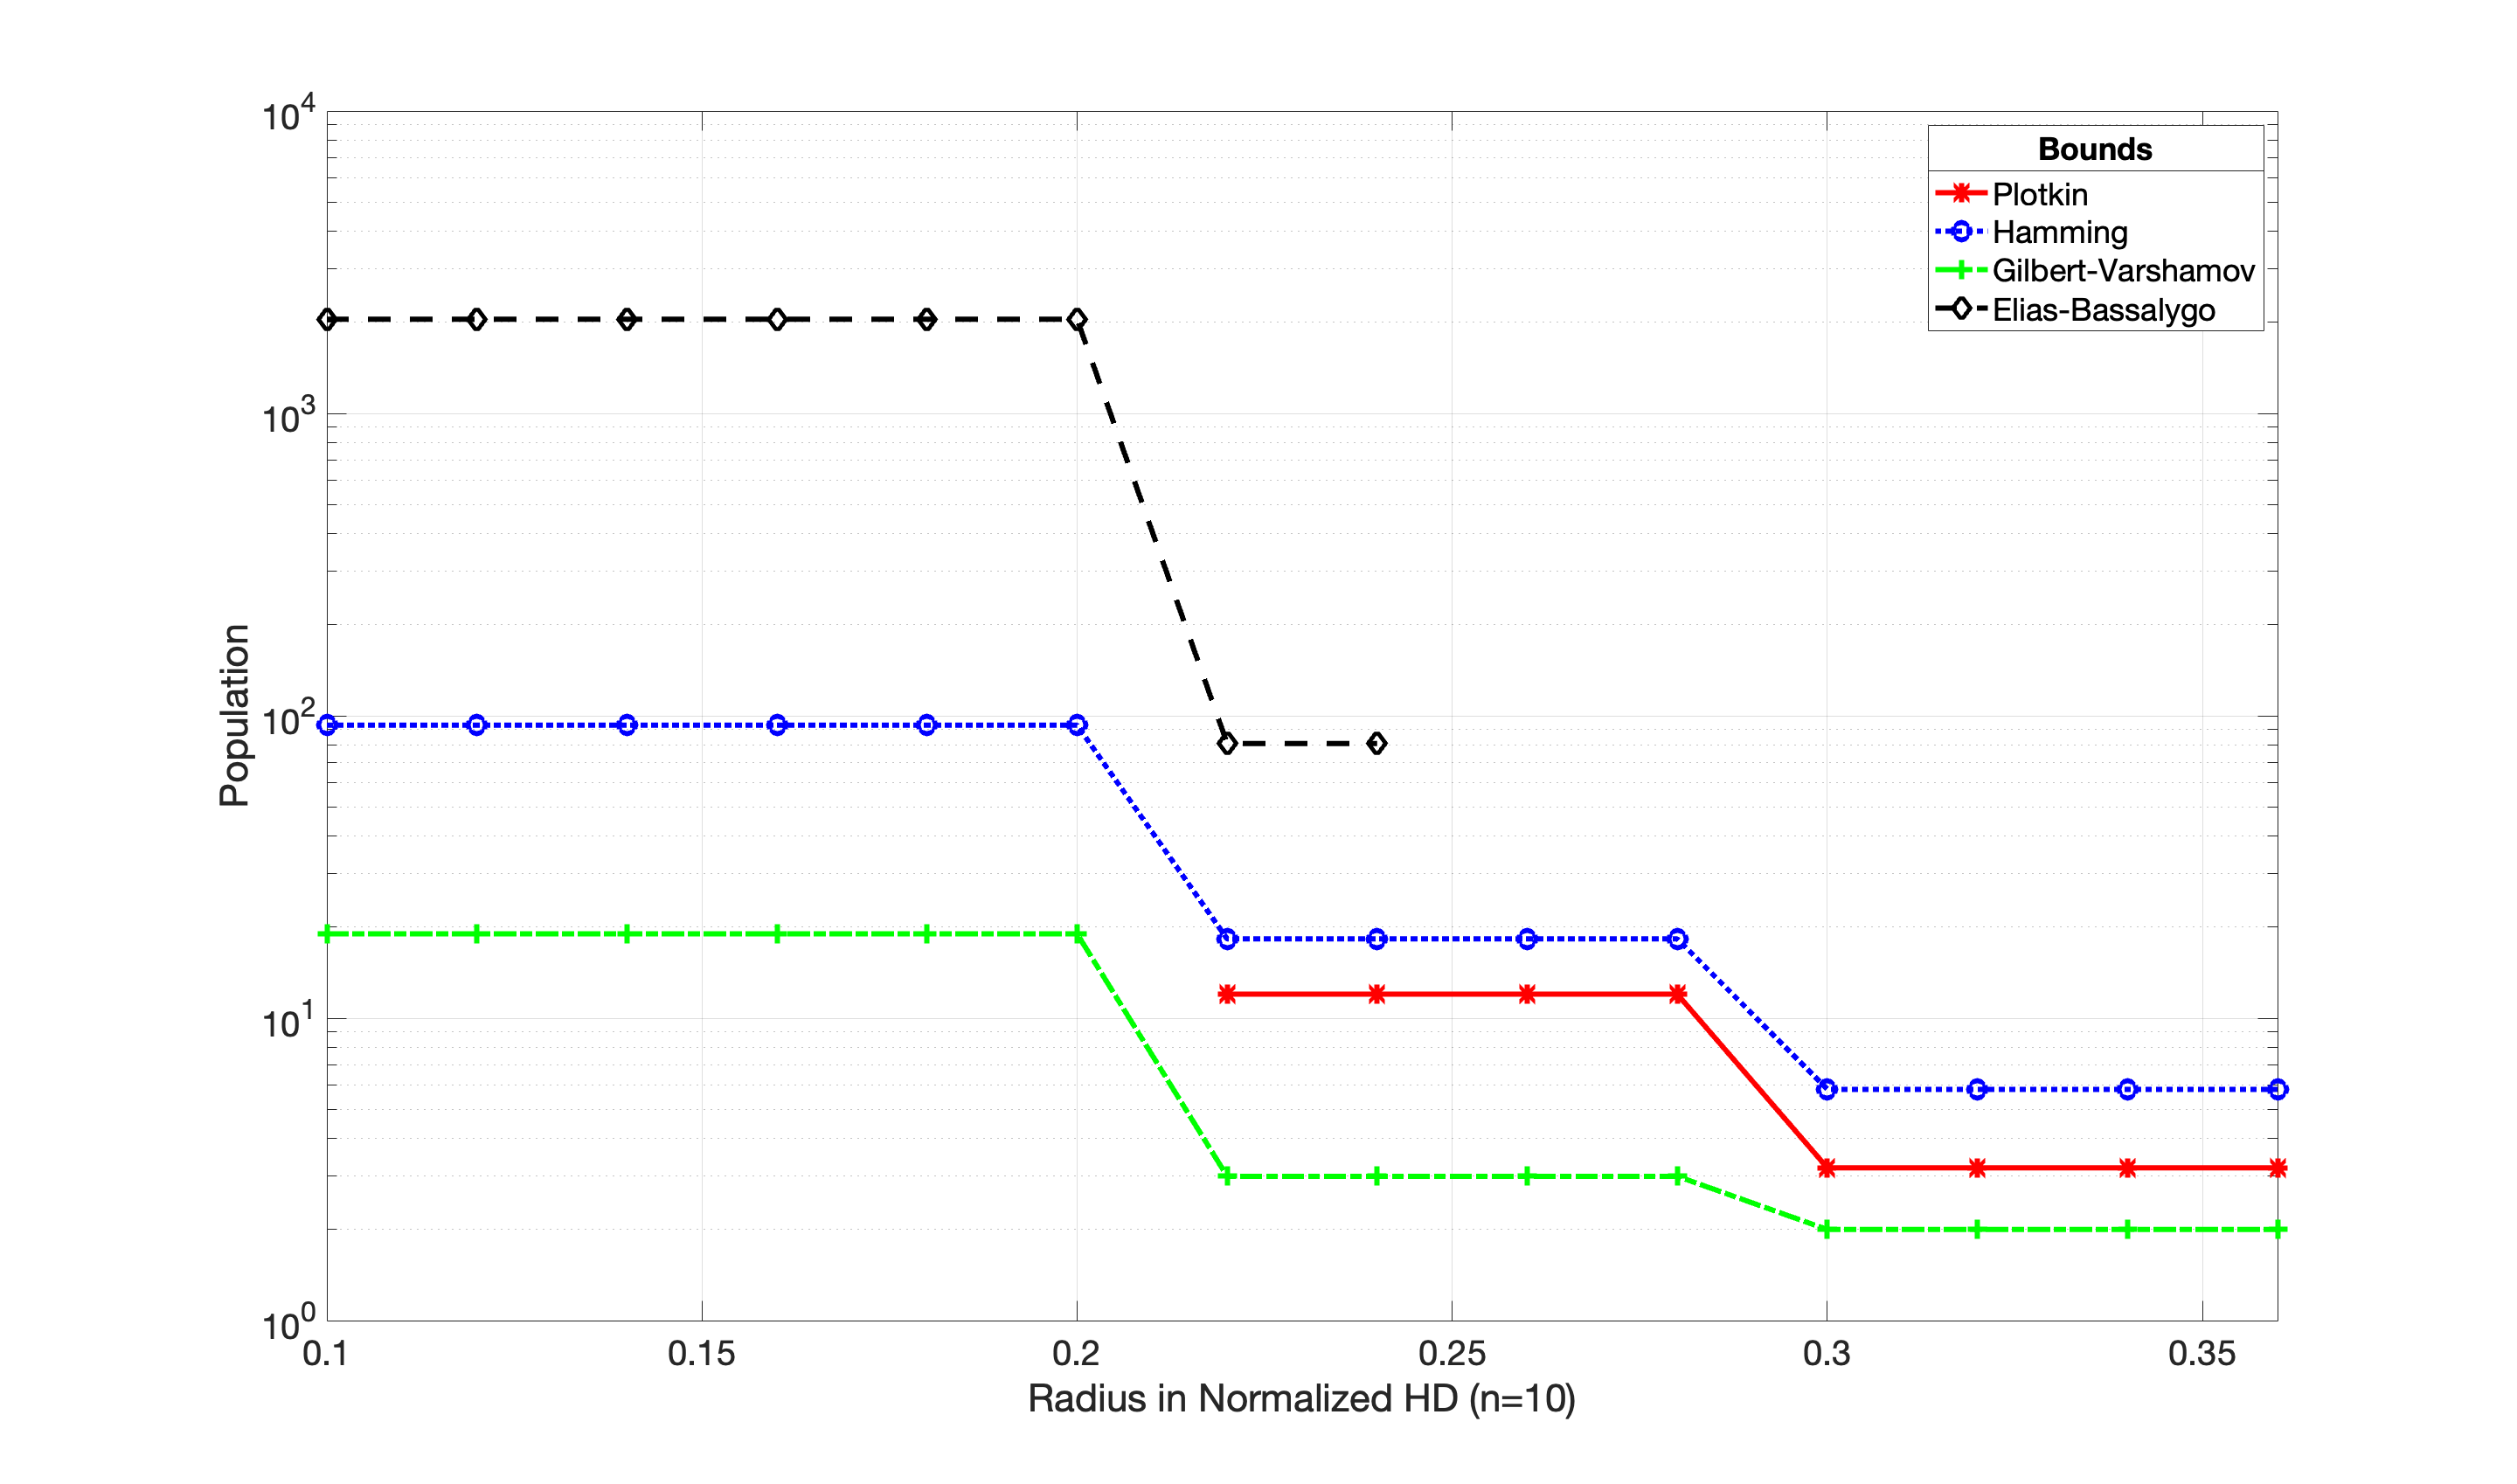
\includegraphics[width=\linewidth]{hw5_figures/10.png}
    \centering
    \caption{Population bounds vs. normalized Hamming distance ($n=10$)}
\end{figure}
\hrule

\paragraph*{Problem 5.1} \hfill\newline
\begin{enumerate}[((a))]
    \item
    \begin{align*}
        h(f)&=-\int_0^\infty\lambda e^{-\lambda x}\ln(\lambda e^{-\lambda x})dx\\
        &=-\lambda\ln(\lambda)\int_0^\infty e^{-\lambda x}dx + \lambda^2\int_0^\infty xe^{-\lambda x} dx\\
        &=-\ln(\lambda)+1
    \end{align*}
    \item
    \begin{align*}
        h(f)&=-\int_{-\infty}^\infty\frac{1}{2}\lambda e^{-\lambda |x|}\ln(\frac{1}{2}\lambda e^{-\lambda |x|})dx\\
        &=-\frac{\lambda}{2}\ln(\frac{\lambda}{2})\int_{-\infty}^\infty e^{-\lambda |x|}dx + \frac{\lambda^2}{2}\int_{-\infty}^\infty |x|e^{-\lambda |x|} dx\\
        &=-\ln(\frac{\lambda}{2})+1
    \end{align*}
    \item Sum of two Gaussians, is again a Gaussian: $X_1+X_2\sim\mathcal{N}(\mu_1+\mu_2, \sigma_1^2+\sigma_2^2)$
    \begin{align*}
        h(f_{X1+X_2})=\frac{1}{2}\ln(2\pi(\sigma_1^2+\sigma_2^2))+\frac{1}{2}
    \end{align*}
\end{enumerate}
\hrule

\paragraph*{Problem 5.2} \hfill\newline
\begin{align*}
    I(X;Y) &= h(X) + h(Y) - h(X, Y)\\
    &=\frac{1}{2}\ln(2\pi \sigma^2)+\frac{1}{2}\ln(2\pi \sigma^2)-\frac{1}{2}\ln((2\pi )^2det(\Sigma))\\
    &=\frac{1}{2}\ln(2\pi \sigma^2)+\frac{1}{2}\ln(2\pi \sigma^2)-\frac{1}{2}\ln((2\pi )^2\sigma^4(1-\rho^2))\\
    &=-\frac{1}{2}\ln(1-\rho^2)
\end{align*}
\begin{itemize}
    \item $\mathbf{\rho=1}$: 
    
    $I(X;Y)=\infty$. $X$ and $Y$ are completely correlated, and their mutual information explodes. (Degenerate Gaussian)
    \item $\mathbf{\rho=0}$: 
    
    $I(X;Y)=0$. $X$ and $Y$ are independent. (And as a result, they are uncorrelated too. In the special case of Multivariate Gaussian, uncorrelated-ness and independence are the same thing)
    \item $\mathbf{\rho=-1}$: 
    
    $I(X;Y)=\infty$. $X$ and $Y$ are completely correlated, and their mutual information explodes. (Degenerate Gaussian)
\end{itemize}
\hrule

\paragraph*{Problem 5.3} \hfill\newline
For this simple distribution we are able to derive mean squared error analytically and take the derivative to find where its minimum value will occur.
\begin{align*}
    E[(x-x')^2]&=\int_{-\infty}^0 \frac{1}{\sqrt{2\pi\sigma^2}} e^{-x^2/\sigma^2}(x+\hat{x})^2dx +\int_0^\infty \frac{1}{\sqrt{2\pi\sigma^2}}e^{-x^2/\sigma^2}(x-\hat{x})^2dx\\
    &=\hat{x}^2+\sigma^2-\frac{4\hat{x}\sigma^2}{\sqrt{2\pi\sigma^2}}
\end{align*}
Now taking the derivative with respect to $\hat{x}$:
\begin{align*}
    \frac{\partial}{\partial\hat{x}}E[(x-x')^2]&=2\hat{x}-\frac{4\sigma^2}{\sqrt{2\pi\sigma^2}}=0\\
    &\hat{x}=\sigma\sqrt{\frac{2}{\pi}}
\end{align*}
So if $X\geq0$ it will be quantized to $\sigma\sqrt{\frac{2}{\pi}}$, otherwise to $-\sigma\sqrt{\frac{2}{\pi}}$.

By substituting back to the expected squared error we can find distortion amount of this quantization scheme:
\begin{align*}
    D=E[(x-x')^2]=(\sigma\sqrt{\frac{2}{\pi}})^2+\sigma^2-\frac{4\sigma\sqrt{\frac{2}{\pi}}\sigma^2}{\sqrt{2\pi\sigma^2}}=\frac{\pi-2}{\pi}\sigma^2
\end{align*}

The distortion bound for a rate of 1 bit, has the value of $0.25\sigma^2$, while the actual distortion we have calculated here is $0.36\sigma^2$ which has, as expected, higher value than the lower bound.\\
\hrule

\paragraph*{Problem 5.4} \hfill\newline
The general rate distortion objective is:
\begin{align*}
    R(D)=\min_{p(\hat{x}|x):Distortion<D} I(X;\hat{X}) 
\end{align*}
By assuming conditional probabilities as $p(0|0)=\alpha$ and $p(1|1)=\beta$ the other conditional probabilities will be calculated as $p(1|0)=1-\alpha$ and $p(0|1)=1-\beta$. \\
The distortion can be written as:
\begin{align*}
    Distortion&=\sum p(x,\hat{x})d(x, \hat{x})\\
    &=\sum p(x)p(\hat{x}|x)d(x,\hat{x})\\
    &=\frac{1}{2}(1-\alpha)2+\frac{1}{2}(1-\beta)1 + \frac{1}{2}(\alpha)0+ \frac{1}{2}(\beta)0\\
    &=\frac{1-\alpha}{2}2+\frac{1-\beta}{2}
\end{align*}
and for the mutual information:
\begin{align*}
    I(X;\hat{X})=H(\hat{x)}-H(\hat{x}|x)=H(\frac{1+\alpha-\beta}{2}, \frac{1-\alpha+\beta}{2})-\frac{1}{2}[H(\alpha, 1-\alpha) + H(\beta, 1-\beta)]
\end{align*}
By using Lagrange multipliers, the final objective will be:
\begin{align*}
    J=H(\frac{1+\alpha-\beta}{2}, \frac{1-\alpha+\beta}{2})-\frac{1}{2}[H(\alpha, 1-\alpha) + H(\beta, 1-\beta)]+\lambda(\frac{1-\alpha}{2}2+\frac{1-\beta}{2}1)
\end{align*}
By setting the derivative equal to zero, we will have 3 equations to be solved simultaneously, and then optimal $\alpha$ and $\beta$ will be found. Then by resubmitting those three values into mutual information we will get the rate as a function of distortion.
\begin{align*}
    \log\frac{(1-\alpha+\beta)/2}{(1+\alpha-\beta)/2}-\log\frac{1-\alpha}{\alpha}-2\lambda=0\\
    -\log\frac{(1-\alpha+\beta)/2}{(1+\alpha-\beta)/2}-\log\frac{1-\beta}{\beta}-\lambda=0\\
    \frac{1-\alpha}{2}2+\frac{1-\beta}{2}=D
\end{align*}
\hrule

\paragraph*{Problem 5.5} \hfill\newline
\begin{enumerate}[((a))]
    \item
    \begin{align*}
        D(f_1||f_2)&=\int_{-\infty}^\infty\frac{1}{\sqrt{2\pi\sigma_1^2}} e^{-x^2/\sigma_1^2}[\frac{1}{2}\ln(\frac{\sigma_2^2}{\sigma_1^2})-\frac{x^2}{2\sigma_1^2}+\frac{x^2}{2\sigma_2^2}]dx\\
        &=\frac{1}{2}\ln(\frac{\sigma_2^2}{\sigma_1^2})+\frac{1}{2}\frac{\sigma_1^2}{\sigma_2^2}-\frac{1}{2}
    \end{align*}
    \item
    \begin{align*}
        D(f_1||f_2)&=\int_0^\infty\lambda_1 e^{-\lambda_1 x}[\ln(\frac{\lambda_1}{\lambda_2})-\lambda_1x+\lambda_2x]dx\\
        &=\ln(\frac{\lambda_1}{\lambda_2})+\frac{\lambda_2}{\lambda_1}-1
    \end{align*}
    \item 
    \begin{align*}
        D(f_1||f_2)&=\int_0^a1\times\ln(\frac{1}{0})+\int_a^11\times\ln(\frac{1}{1})\\
        &=\infty
    \end{align*}
    \item 
    \begin{align*}
        D(f_1||f_2)&=\frac{1}{2}\times\ln(\frac{1/2}{1})+\frac{1}{2}\times\ln(\frac{1/2}{0})\\
        &=\infty
    \end{align*}
\end{enumerate}
\hrule

\paragraph*{Problem 5.6} \hfill\newline
\begin{enumerate}[((a))]
    \item
    \begin{align*}
        D(p_0||p_1)&=\sum p_0(x)\log(\frac{p_0(x)}{p_1(x)})\\
        &=\sum (\frac{1}{2})^x\log(\frac{(\frac{1}{2})^x}{qp^{x-1}})\\
        &=\sum (\frac{1}{2})^x(-x\log(2p)) + \sum (\frac{1}{2})^x\log(\frac{p}{q})\\
        &=\log(\frac{1}{4p^2})+\log(\frac{p}{q})\\
        &=-\log(4pq)
    \end{align*}

    \item
    The exponent of error (Chernoff Information) is as follows:
    \begin{align*}
        -\min_{0\leq\lambda\leq1}\log(\sum p_0^\lambda(x) p_1^{1-\lambda}(x))
    \end{align*}
    The expression will be a function of $\lambda$:
    \begin{align*}
        \sum p_0^\lambda(x) p_1^{1-\lambda}(x)&=(\frac{q}{p})^{1-\lambda}\sum(\frac{p^{1-\lambda}}{2^\lambda})^x\\
        &=\frac{p^\lambda q^{1-\lambda}}{(2p)^\lambda-p}
    \end{align*}
    after taking the $\log$ of the above expression, now we take the derivative of objective function and set it to zero:
    \begin{align*}
        -\log(q)+\log(p)-\frac{1}{(2p)^\lambda-p}(2p)^\lambda\log2p=0\\
        \lambda=\frac{1}{\log2p}\log(\frac{\log q/p}{\log 2q})
    \end{align*}
\end{enumerate}
\hrule

\paragraph*{Problem 5.7} \hfill\newline
From Sanov's theorem we knew that:
\begin{align*}
    Pr(\frac{1}{n}\sum X_i^2\geq\alpha^2)\doteq e^{-n \inf_{P*\in\mathcal{E}}D(P*||\mathcal{N}(0,1))}
\end{align*}
by taking $\log$ from both sides, we will have the exponent:
\begin{align*}
    D(P^*||Q)&=-\frac{1}{n}\log Pr(\frac{1}{n}\sum X_i^2\geq\alpha^2)\\
    D(P^*||Q)&=\int f(x)\ln\frac{f(x)}{\frac{1}{\sqrt{2\pi \sigma^2}}e^{-\frac{x^2}{2\sigma^2}}}dx\\
    &=-h(f) + \frac{1}{2\sigma^2}\mathbb{E}[X^2] + \frac{1}{2}\ln2\pi\sigma^2
\end{align*}
As relative entropy always is greater than zero, to have $D(P^*||Q)$ minimized, we need the $h(f)$ to be maximized. Among all continuous random variables, Gaussian random variable has the maximum entropy, so  $f=\mathcal{N}(0, \alpha^2)$.

Therefore we have the minimum value exponent of Sanov's equation, as:
\begin{align*}
    D(P^*||Q)&=-\frac{1}{2}\ln(2\pi\alpha^2)-\frac{1}{2}+\frac{\alpha^2}{2\sigma^2} + \frac{1}{2}\ln2\pi\sigma^2\\
    &=\frac{\alpha^2}{2\sigma^2} + \frac{1}{2}\ln\frac{\sigma^2}{\alpha^2}-\frac{1}{2}
\end{align*}

\hrule

\newpage
\paragraph*{Appendix} \hfill\newline
\begin{lstlisting}[caption = {Matlab Code to Plot Bounds}]
clc;
clear all;
close all;

n = 245;
number_of_points = 14;

%% Hamming Bound

e = 0.10;
hamx = zeros(number_of_points);
hamy = zeros(number_of_points);
syms j;

for i = 1:number_of_points
    r = floor(n*e);
    d = (2 * r) + 1;
    hamx(i) = e;
    hamy(i) = 2^n / symsum(nchoosek(n, j), j, 0, r);
    e = e + 0.02;
end

%% Plotkin Bound

e = 0.10;
plotkinx = zeros(1,number_of_points);
plotkiny = zeros(1,number_of_points);

for i = 1:number_of_points
    r = n * e;
    r = floor(r);
    d = (2 * r) + 1;
    plotkinx(i) = e;
    if mod(d,2) == 0 && (2 * d) > n
        plotkiny(i) = 2*(d/(2*d)-n);
    elseif mod(d,2) == 1 && (2*d) + 1 > n
        plotkiny(i) = 2 * ((d + 1) / ((2 * d) + 1 - n));
    elseif mod(d,2) == 0 && 2 * d == n
        plotkiny(i) = 4 * d;
    elseif mod(d,2) == 1 && (2 * d) + 1 == n
        plotkiny(i) = (4 * d) + 4;
    else 
            disp("not valid.");
    end  
    e = e + 0.02;
end 

%% Elias-Bassalygo Bound

e = 0.10;
ebx = zeros(number_of_points);
eby = zeros(number_of_points);

for i=1:8
    r = floor(n * e);
    d = (2 * r) + 1;
    ebx(i) = e;
    Jnr = floor((n / 2) * (1 - sqrt(1 -((2 * (2 * r + 1)) / n))));
    eby(i) = floor((n * 2^(n + 1)) / nchoosek(n, Jnr));

    e = e + 0.02;
end

%% Gilbert-Varshamov Lower Bound

e = 0.10;
gvx = zeros(number_of_points);
gvy = zeros(number_of_points);

for i = 1:number_of_points
    r = floor(n * e);
    d = (2 * r) + 1;
    gvx(i) = e;
    gvy(i) = ceil((2^n) / symsum(nchoosek(n, j), j, 0, 2 * r));
    e = e + 0.02;
end


%% Plotting

h0 = semilogy(plotkinx, plotkiny, 'r-*','LineWidth', 3, 'MarkerSize',10);
hold on;

h1 = semilogy(hamx, hamy, 'b:o','LineWidth', 3, 'MarkerSize',10);
h2 = semilogy(gvx, gvy, 'g-.+','LineWidth', 3, 'MarkerSize',10);
h3 = semilogy(ebx, eby, 'k--d','LineWidth', 3, 'MarkerSize',10);

lgd = legend([h0, h1(1), h2(1), h3(1)], 'Plotkin', 'Hamming', 'Gilbert-Varshamov', 'Elias-Bassalygo');
title(lgd,'Bounds');
grid on;
xlim([0.10 0.36]);
set(gca,'FontSize',20);
ylabel('Population');
xlabel(sprintf('Radius in Normalized HD (n=%d)', n));

\end{lstlisting}
\end{document}


